\section{Adjusted mutual information analysis}
	This section summarizes the adjusted mutual information project
	
	
	\subsection{Purpose}
	
		The purpose is the same than for the Photonic Lanter Information Determination with euclidean distances, but this time instead of looking at pairs of points we look at clusters of points to see how their relationship evolve along the optical pathway.\\
		
		To do this we create datasets generated from 2, 5, 9, 14, 20, 27, 35 and 44 zernike modes.\\
		
		When the datasets are created we use K-Means clustering to group points and measure the conservation of energy using the adjusted mutual information score.\\
		
		After this, we also check how the adjusted mutual information changes with datasets of different sizes generated with 9 zernike modes.
		
		
	\subsection{The data}
		There are 4 different types of datasets:
		\begin{itemize}
			\item Zernike coefficients
			\item PSF
			\item LP coefficients
			\item Photonic Lantern Output fluxes
		\end{itemize}
		
		The paths to the datasets can be found in \href{https://github.com/Dacarpe03/PLImageReconstruction/blob/main/Utils/nmi_analysis_constants.py}{nmi\_analysis\_constants.py} which contain the information for the 5000 datapoints datasets for 2, 5, 9, 14, 20, 27, 35 and 44 zernike modes.
		
		The second set of paths to the datasets used to check how the AMI evolves with the number on points of the dataset can be found in \href{https://github.com/Dacarpe03/PLImageReconstruction/blob/main/Utils/ami_analysis_constants.py}{ami\_analysis\_constants.py}.
		
	
	\subsection{Results}
		\begin{figure*}[ht!]
			\centering
			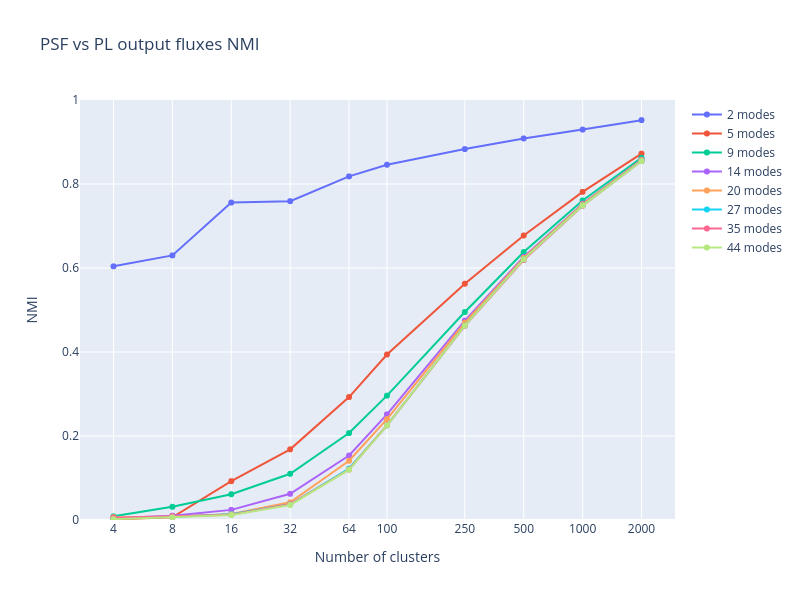
\includegraphics[width=0.9\textwidth]{nmia-psfvsploutputfluxesnmi.png}
		\end{figure*}
		\FloatBarrier
		
		The conservation of information decreases over the number of Zernike modes, this could be improved by measuring the outputs of the photonic lantern in different wavelengths.\\
		
		\begin{figure*}[ht!]
			\centering
			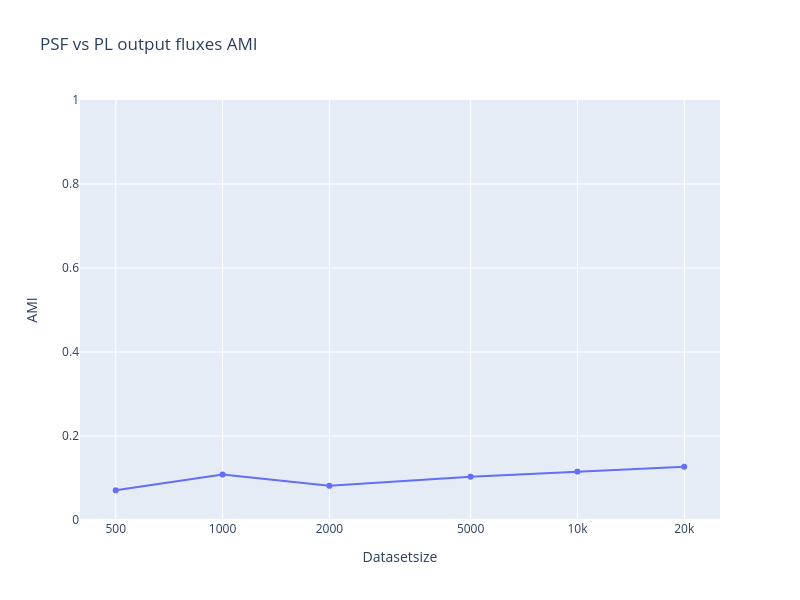
\includegraphics[width=0.9\textwidth]{ld-psfvsploutputfluxesami.png}
		\end{figure*}
		\FloatBarrier
		
		The AMI improves slightly as the number of datapoints increase, this could be because the clusters are more dense and the information locally is better conserved than globally.\\
		
		These results are not what we expected so we looked at the AMI between LP complex coefficients and complex amplitudes of the photonic lantern:
		
		\begin{figure*}[ht!]
			\centering
			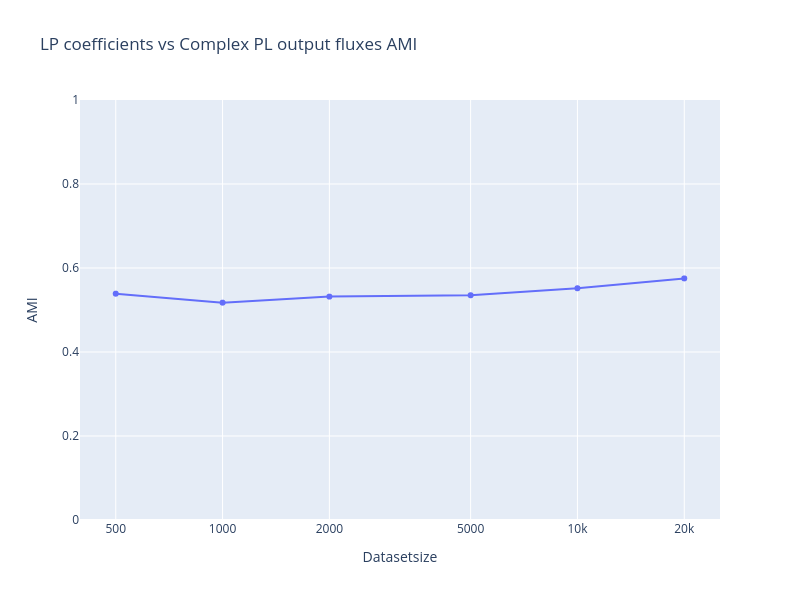
\includegraphics[width=0.9\textwidth]{ld-lpcoefficientsvscomplexploutputfluxesami.png}
		\end{figure*}
		\FloatBarrier
		The AMI between them should be very high but it is not so there is either a problem with the transfer matrix or the clustering (which could be losing information).
		
	
	\subsection{Code}
	
	Code for AMI analysis over number of Zernike modes
	\begin{itemize}
		\item The data generation for the AMI analysis over number of Zernike Modes can be found in \href{https://github.com/Dacarpe03/PLImageReconstruction/blob/main/PSFReconstruction/DataNotebooks/NMIAnalysisDatasetZernikePSFGeneration-Copy1.ipynb}{NMIAnalysisDatasetZernikePSFGeneration-Copy1.ipynb}
		\item The data processing for the AMI analysis over number of Zernike Modes can be found in \href{https://github.com/Dacarpe03/PLImageReconstruction/blob/main/PSFReconstruction/DataNotebooks/NMIAnalysisdatasetProcessing.ipynb}{NMIAnalysisdatasetProcessing.ipynb}
		\item The dimensionality reduction of the data for the AMI analysis over number of Zernike Modes can be found in \href{https://github.com/Dacarpe03/PLImageReconstruction/blob/main/PSFReconstruction/DataNotebooks/NMIAnalysisDatasetDimensionalityReduction.ipynb}{NMIAnalysisDatasetDimensionalityReduction.ipynb}
		\item The clustering of the data for the AMI analysis over number of Zernike Modes can be found in \href{https://github.com/Dacarpe03/PLImageReconstruction/blob/main/PSFReconstruction/DataNotebooks/NMIAnalysisDatasetClustering.ipynb}{NMIAnalysisDatasetClustering.ipynb}
		\item The plots and AMI analysis over number of Zernike Modes can be found in \href{https://github.com/Dacarpe03/PLImageReconstruction/blob/main/PSFReconstruction/DataNotebooks/NMIAnalysisOverNClusters.ipynb}{NMIAnalysisOverNClusters.ipynb}
	\end{itemize}
	
	Code for AMI analysis over dataset size:
	\begin{itemize}
		\item The data generation for the AMI analysis over dataset size can be found in \href{https://github.com/Dacarpe03/PLImageReconstruction/blob/main/PSFReconstruction/Scripts/LastDanceDatasetZernikePSFGeneration.py}{LastDanceDatasetZernikePSFGeneration.py}
		\item The data processing for the AMI analysis over dataset size can be found in \href{https://github.com/Dacarpe03/PLImageReconstruction/blob/main/PSFReconstruction/Scripts/LastDancedatasetProcessing.py}{LastDancedatasetProcessing.py}
		\item The dimensionality reduction of the data for the AMI analysis over dataset size can be found in \href{https://github.com/Dacarpe03/PLImageReconstruction/blob/main/PSFReconstruction/Scripts/LastDanceDatasetDimensionalityReduction.py}{LastDanceDatasetDimensionalityReduction.py}
		\item The clustering of the data for the AMI analysis over dataset size can be found in \href{https://github.com/Dacarpe03/PLImageReconstruction/blob/main/PSFReconstruction/Scripts/LastDanceDatasetClustering.py}{LastDanceDatasetClustering.py}
		\item The plots and AMI analysis over number of Zernike Modes can be found in \href{https://github.com/Dacarpe03/PLImageReconstruction/blob/main/PSFReconstruction/DataNotebooks/LastDanceAMIAnalysisOverNClusters.ipynb}{LastDanceAMIAnalysisOverNClusters.ipynb}
	\end{itemize}
	
	\subsection{Detailed results}
		For a detailed report on the datasets, results and plots see Part VIII from \filename{all.pdf}.